\section*{13. How to Mine with NiceHash }
\addcontentsline{toc}{chapter}{How to Mine with NiceHash }

The easiest way to get started at mining is with NiceHash. NiceHash launched in 2014, right around the time of the first major spike in cryptocoin mining (second if you want to include Bitcoin's initial surge to \$32 per BTC in 2011). Prior to NiceHash, getting started with coin mining was quite a bit more complicated — as we'll detail below. NiceHash has greatly lowered the barrier to entry, and it gets rid of some of the worries about what coin(s) to mine. You effectively lease your PC's hashing power to other users, who get to choose what to mine, and you get paid in Bitcoin. NiceHash takes a small cut of the potential profits, and your PC can be up and mining in minutes.\vspace{.3cm}

\begin{figure}[h]
	\centering
	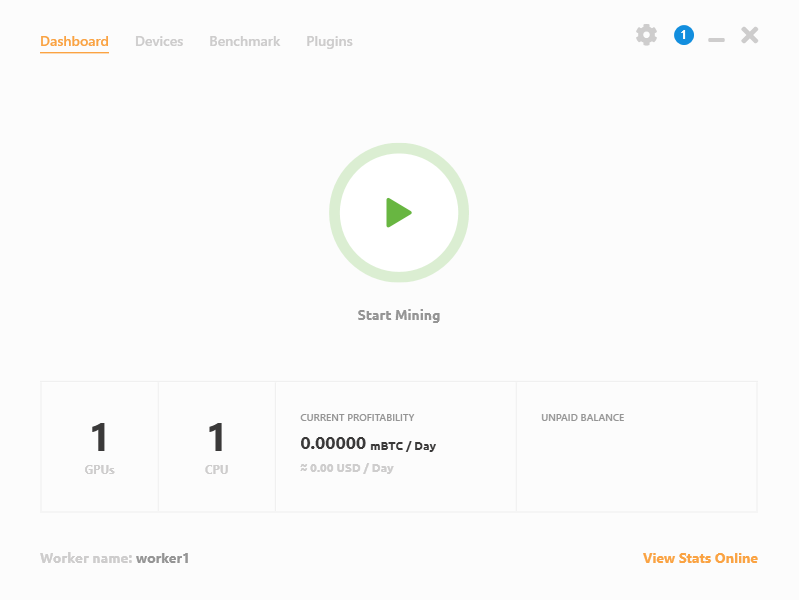
\includegraphics[width=0.7\linewidth]{Screenshot (4)}
	\captionsetup{labelformat=empty}
	\caption{Nicehash Miner}
\end{figure}

NiceHash has several options, ranging in degree of complexity. The easiest is to use the new QuickMiner, which is a web interface to a basic mining solution. You download the QuickMiner software, run that, and the webpage allows you to start and stop mining — you don't even need to put in your BTC address. It's dead simple, though the numbers can fluctuate quite a bit. For example, in a brief test QuickMiner suggested it was earning over \$7 per day (on an RTX 3090), and noted we "could be making 16\% more" by using NiceHashMiner (which we'll get to next). Except, after letting both versions run for a bit, QuickMiner seemed to stabilize at the same performance level as NiceHashMiner. YMMV.\vspace{.3cm}

Next up is NiceHashMiner, which is what most people will want to use. It's more complex in some ways than QuickMiner, but it has more options that can improve overall profitability. By default, it will ask you to log in using your NiceHash account details. Alternatively, you can use the NiceHash app on your phone to scan a QR code, or just input your BTC address manually.\vspace{.3cm}

Once launched, the first time it runs, NiceHashMiner will benchmark your hardware using various common mining (hashing) algorithms. Which algorithms and software get tested varies a bit by your GPU, and you can customize things quite a bit. Right now, DaggerHashimoto (aka, Ethash, what Ethereum uses — a modified variant of DaggerHashimoto) tends to be the most profitable, though sometimes Octopus or some other algorithm might sneak in some cycles.\vspace{.3cm}

The idea is that NiceHashMiner will choose whatever is currently the most profitable coin to mine, based on what people are willing to pay to lease your hardware. Sometimes a new coin will launch, or someone will want to dedicate a lot of mining power at a specific coin, and they'll pay more to do so. Instead of mining Ethereum 24/7, you might occasionally run some other algorithm, and it's all managed by the software, which usually (but not always) manages to do a good job.\vspace{.3cm}

The initial benchmarks on NiceHashMiner can be a bit prone to error, unfortunately. That's because the tests are only run for a minute each, and as your GPU heats up it may also slow down. That means the first algorithm benchmarked often ends up with an inflated result. You can get a better estimate of performance by using the Precise mode (on the benchmark tab), which takes twice as long to benchmark. You can also manually enter hash rates, so for example if you notice that after 30 minutes or more that NBminer stabilizes at 94MH/s instead of 98MH/s, you can fine tune the mining speed. You can also schedule an algorithm for retesting if you think the result is off, and by default (it can be turned off) NiceHashMiner will periodically download new versions of the miners and automatically retest.\vspace{.3cm}

\subsection*{13.1 What are the benefits?}

NiceHash Miner is an advanced auto-miner that supports the latest algorithms and miners. No need to go through tons of configuration files, various mining software versions, configuration tuning or cryptocurrency coins market analysis. Auto-tuning for best performance and efficiency, automatic selection and runtime automatic switching to most profitable cryptocurrency algorithm are all integrated into NiceHash Miner and will enable you seamless, joyful and profitable mining experience.\vspace{.3cm}

\subsection*{13.2 Features}
\begin{itemize}
	\item Easy one-click CPU mining for CPUs that support at least AES (only works on Windows x64).
	\item Easy one-click GPU mining for NVIDIA GPUs using microarchitecture (compute capability) SM 3.0+.
	\item Easy one-click GPU mining for AMD GPUs using any AMD GPU devices that supports OpenCL.
	\item Integrated support for Simple Multi-Algorithm. Always mine most profitable algorithm.
	\item Integrated benchmarking tool. Run it only once before you start mining and after every hardware/driver/software upgrade.
	\item Watch-feature - automatically restart miner if crashed or hanged.
	\item Display current rate and your balance in real time.
	\item Auto update notifications.
	\item Much more...
\end{itemize}

\subsection*{13.3 Requirements}
\begin{itemize}
	\item Windows 10 or newer operating system 64-bit
	\item Windows 10 is recommended and will provide you a much better user experience
	\item For CPU mining a modern CPU with AES support
	\item For AMD mining any AMD GPU with OpenCL support
	\item For NVIDIA mining any NVIDIA GPU with Compute capability (SM) 3.0 or newer
	\item up-to-date patches for OS
	\item up-to-date drivers for all GPUs
	\item Reliable internet connectivity
	\item For GPU Mining, paging file size of 60\% of your total GPU VRAM memory
	\item Personal Bitcoin wallet (you can create one by registering on NiceHash page)
\end{itemize}

\subsection*{13.4 How to get\&run it?}
All you have to do is download zip package or installer exe from the releases page. If you choose installer just run it and follow the instructions. In case of zip package extract it and run the miner. After that enter your Bitcoin wallet address where you want to get your coins sent at - and you are ready to start mining and maximizing your profit.\vspace{.3cm}

Note: Windows 10 with .NET Framework 4.8 or higher and Microsoft Visual C++ Redistributable 2015 are required. However, if you encounter any issues when starting application (application would fail to start or errors/warnings about missing DLL files are displayed) you should download and install Microsoft .NET Framework 4.8 and Microsoft Visual C++ Redistributable 2015 (vcredist\_x64.exe) (after installation a reboot might be required).\vspace{.3cm}

Detailed instructions:\vspace{.3cm}
\begin{itemize}
	\item Download binaries from here: https://github.com/nicehash/NiceHashMiner/releases
\begin{itemize}
	\item Installer
\begin{itemize}
	\item Run installer file (nhm\_windows\_3.x.y.z.exe)
	\item Follow the instructions
\end{itemize}
\item Zip archive
\begin{itemize}
	\item Extract zip archive
	\item Run NiceHashMiner.exe
\end{itemize}
\end{itemize}
Make sure you select your own personal Bitcoin wallet to receive payments, see Bitcoin wallet guidelines and instructions here:\\ https://www.nicehash.com/support/general-help/wallet/how-to-use-nicehash-wallet.
You will receive Bitcoin payments according to our payments schedule:\\ https://www.nicehash.com/support/mining-help/earnings-and-payments/when-and-how-do-you-get-paid

\end{itemize}

The third and final NiceHash option is to use NiceHash OS. This is a custom Linux installation that would run in place of Windows, and it's recommended for larger scale mining farms that use NiceHash. As with all things Linux, getting it up and running may require a bit more knowledge and patience, but because it's an OS tuned specifically for mining, hash rates can be higher. (We didn't do any of our testing with NiceHash OS, due to time constraints.)\vspace{.3cm}

There are two big downsides to mining via NiceHash. One is that you're not actually getting Ethereum — not directly, at least. You'll get paid in Bitcoin, which you can then trade for Ethereum if you want. That's not necessarily a bad thing, considering BTC is the largest of cryptocoins, but if you want ETH you'll need to take some extra steps. The other downside is that NiceHash takes a cut of the amount paid, and the net result is generally lower payouts than mining Ethereum yourself. How big is the difference? Currently, direct Ethereum mining should pay about 7\% more than NiceHash. That's a pretty big mining fee, though again the ease of use with NiceHash is hard to overstate.\vspace{.3cm}

\subsection*{13.5 Where is the profit coming from?}
As a back-end NiceHash Miner relies on the NiceHash.com service. By running NiceHash Miner you're essentially selling the hashing power of your CPUs \& GPUs to hashing power buyers. Those are using the hashing power to mine various cryptocurrency coins and support decentralized blockchain networks - similar to cloud computing - only that by running NiceHash Miner you're actually being a provider for the cryptocurrency mining hashing power. You are being part of a global compute power network, empowering decentralized digital currencies.
\begin{figure}[h]
	\centering
	\includegraphics[width=1\linewidth]{"images/Screenshot (15)"}
	\captionsetup{labelformat=empty}
	\caption{}
\end{figure}
\pagebreak
\subsection*{13.6 How to run NiceHash Miner only when profitability is high enough?}
Profitability of mining can go up and down that may be unprofitable to mine especially places with high electricity cost. By using the "MinimumProfit" settings, NiceHashMiner will stop mining if the current profits are below the minimum amount (in USD). This will help you mine during "profitable" times only.
\begin{figure}[h]
	\centering
	\includegraphics[width=1\linewidth]{"images/Screenshot (14)"}
	\captionsetup{labelformat=empty}\caption{}
\end{figure}



